%chapanalysis.tex
%
\Section{General Overview}%
%
One of the goals of the analysis is to determine the normalized yields from the raw data collected during the experiment. The normalized yield is the number of events that pass a given set of cuts divided by the cumulative charge delivered by the beam and corrected for various inefficiencies of the experimental equipment. We have extracted nuclear transparency by forming a super ratio of the experimental yield to the Monte Carlo simulation yield from given targets with nucleon number $A$ and deuterium. This ratio is shown in the expression below:

\begin{equation} \label{equ:nucltransp}
T = 
{\left( \frac{\bar Y}{\bar Y_{\rm MC}} \right)_A}/
{\left( \frac{\bar Y}{\bar Y_{\rm MC}} \right)_{\rm D}},
\end{equation}

%\begin{center}$$T=\frac{\frac{Yield_A^{data}}{Yield_A^{SIMC}}}{\frac{Yield_0^{data}}{Yield_0^{SIMC}}}$$
%\end{center}

$\bar{Y}$ is experimental charge-normalized data yield and $\bar{Y}_{MC}$ is the charge-normalized Monte Carlo equivalent yield. In this chapter, we will describe the steps involved in extracting the normalized yields and transparency. For determining the nuclear transparency of kaons, we have reconstructed the physical variables $Q^2$, $W$, $t$ and $\phi_{pq}$ for each event at the interaction vertex.
%Where $Q^2$ is four momentum transfered square, W is the center of mass energy, t is momentum transfer in the center of mass frame and $\phi_{pq}$ is  the angle between the scatering and reaction planes.
The measured yield is an integral over all of these variables.

\Section{Particle Identification(PID)}%
%
\label{Particle Identification(PID)}
We have used particle track information from drift chambers, time-of-flight information from scintillators, response from a gas $\breve{C}$erenkov detector and an aerogel $\breve{C}$erenkov detector to identify the kaons and separate them from other hadrons, such as pions and protons.

\SubSection{Tracking}%
The drift chambers provide the position, angle and momentum (relative to the central momentum) of the particles passing through the spectrometer. We have applied cuts on the reconstructed position, angle and momentum to ensure that they are well within the spectrometer acceptance. Due to poor statistics at the edges of the acceptance, tight cuts were applied on these variables to ensure a good match between the data and SIMC yields.

\SubSection{Charge-Normalized Yield}%
The charge normalized yield can be defined as 
\begin{equation}
\bar{Y} = \frac{Y}{Q}
\end{equation}
where $Y$ is the yield of a given run in counts and $Q$ is the charge delivered by beam (in mC), measured by Beam Current Monitors (BCM) and integrated over the time duration of a run. The yield is given by

\begin{equation} \label{equ:yield}
Y = \frac{N_{true}}{[\epsilon_{scer}\epsilon_{track}f_{elec}]_{SOS}[\epsilon_{hcer}\epsilon_{haero}\epsilon_{track}/f_{elec}]_{HMS}}\frac{N_{pretrigger}}{N_{trigger}}\frac{1}{T_h}
\end{equation}

\noindent
where $N_{true}$ is the true number of events, $f_{elec}$ is electronic dead-time correction factor, $\epsilon_{hcre}$ is the HMS $\breve{C}$erenkov efficiency, $\epsilon_{scre}$ is the SOS $\breve{C}$erenkov efficiency, $\epsilon_{aero}$ is the HMS aerogel efficiency, $\epsilon_{track}$ is the HMS/SOS tracking efficiency and $\frac{N_{trigger}}{N_{pretrigger}}$ is the lifetime. The transmission through the target material, the window of the scattering chamber, the windows of the spectrometer, etc. are collectively referred to as $T_h$.

\SubSection{Coincidence Time}%
Coincidence time is defined as the difference of the time taken by the scattered electrons to reach the SOS to the time taken by the hadrons (p, $\pi^+$, $K^+$) to reach the HMS. Good coincidence timing is the most useful and important information used to achieve clean real $K^+$ yield and helps to measure the insufficiencies of the most of the other cuts.

\begin{figure}[!tbp]
  \centering
  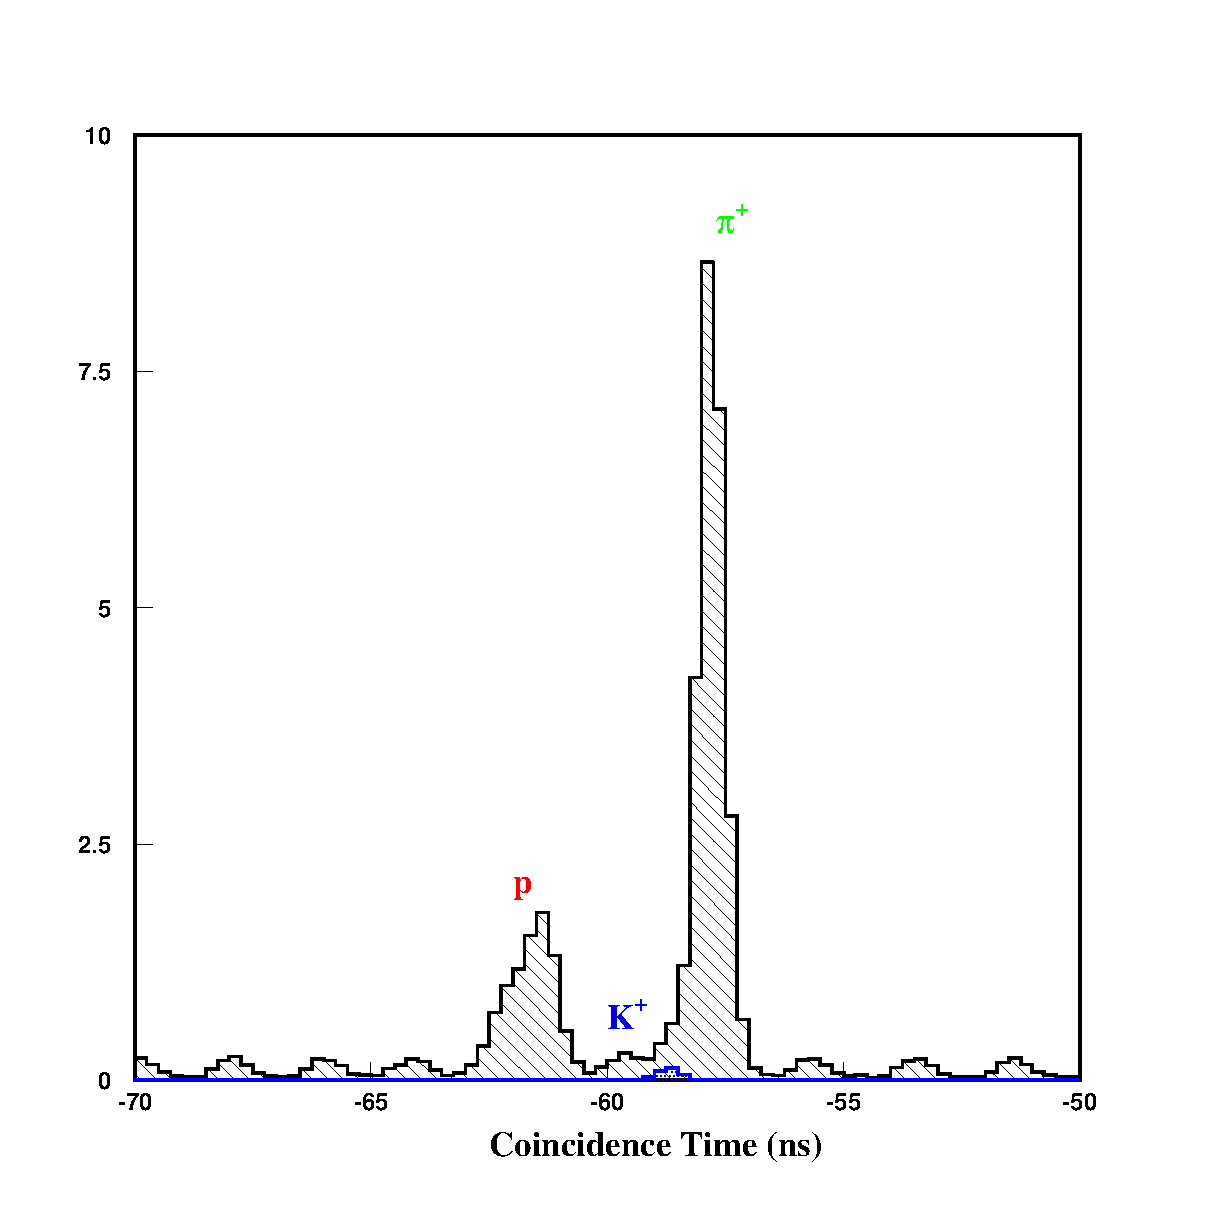
\includegraphics[trim = 1mm 1mm 1mm 1mm,clip,width=0.8\columnwidth]{cointime1}
  \caption[Coincidence time plot of the experiment.]{\label{fig:cointime1}Coincidence time plot of the experiment.\\\\ The broad peak in the right side is from $\pi^+$, proton peak in the left and reasonable number of $K^+$ in the middle shown in BLUE.}
\end{figure}
%\setlength{\figwidth}{0.8\linewidth}
%\Figure{cointime1}{\figwidth}{Coincidence time plot of the experiment. The broad peak in the right side is from $\pi^+$, proton peak in the left and reasonable number of $K^+$ in the middle shown in \textcolor{blue}{BLUE}.}

\begin{figure}[!tbp]
  \centering
  \includegraphics[trim = 1mm 1mm 1mm 1mm,clip,width=0.8\columnwidth]{cointime2}
  \caption[Zoomed coincidence time plot of the experiment.]{\label{fig:cointime2}Zoomed coincidence time plot of the experiment.\\\\ The selected peak of $K^+$ in BLUE in the middle from $\pi^+$ and proton peak in the right and left, respectively, after applying all the cuts.}
\end{figure}
%\setlength{\figwidth}{0.8\linewidth}
%\Figure{cointime2}{\figwidth}{Zoomed coincidence time plot of the experiment. The selected peak of $K^+$ in \textcolor{blue}{BLUE} in the middle from $\pi^+$ and proton peak in the right and left, respectively, after applying all the cuts.}

The time-of-flights (TOF) of the electron in the SOS and of hadrons in the HMS were obtained from the TOF scintillator detectors in each spectrometer. These were used to determine the coincidence time, which is the relative time difference between the electron and the hadron projected back to the target. Cuts on coincidence time were used to separate kaons from pions and protons.

A typical plot of the coincidence time of the experiment is shown in \figureref{cointime1}. Since the experiment was designed for pions, one can see a sharp peak of $\pi^+$ in the 30 ns coincidence window. There is a broad peak of protons as well and between protons and $\pi^+$ peak there is a rather small peak of kaons. In \Figureref{cointime1}, the small periodic peaks at an interval of 2.004 ns are due to the 499 MHz pulse structure of the beam delivered by the accelerator to Hall-C. One of the most effective PID cuts was over coincidence time in order to separate $K^+$ from $\pi^+$ and protons. Selected kaons after applying all the cuts are shown by BLUE region in \Figureref{cointime2}.

The fraction of electron-kaon coincidences that were uncorrelated accidental coincidences must be corrected in order to arrive at the true electro-production yield. The accidental coincidences have been corrected using the average number of kaon events in three of the small peaks that are 2.004 ns apart on both sides of the central coincidence time peak and has been shown by the GREEN band in \figureref{misscoin}.

\SubSection{Missing Mass}%
\label{Missing Mass}
To understand missing mass, we need to look into the basic reactions of the experiment, which can 
be written as
\begin{equation}
\label{L0}
e + p \rightarrow e^\prime + K^+ + \Lambda^0
\end{equation}
\begin{equation}
\label{S0}
e + p \rightarrow e^\prime + K^+ + \Sigma^0
\end{equation}
\begin{equation}
\label{S-}
e + n \rightarrow e^\prime + K^+ + \Sigma^-
\end{equation}
In the nucleus, the reaction can be written as
\begin{equation}
e + A \rightarrow e^\prime + K^+ + \Lambda^0 + X
\end{equation}
\begin{equation}
e + A \rightarrow e^\prime + K^+ + \Sigma^0 + X
\end{equation}
\begin{equation}
e + A \rightarrow e^\prime + K^+ + \Sigma^- + X
\end{equation}
Since the $\Lambda$/$\Sigma$ are not detected, from energy and momentum conservation we can write from Eq. \ref{L0}, \ref{S0} and \ref{S-},\\
Energy conservation: 
\begin{equation}
E_e + M_p = E_{e^\prime} + E_{K^+} + E_X ~\mathrm{or,}~ E_X = E_e + M_p - E_{e^\prime} - E_{K^+}
\end{equation}
Momentum conservation:
\begin{equation}
P_e + 0 = P_{e^\prime} + P_{K^+} + P_X ~\mathrm{or,}~ P_X = P_e + 0 - P_{e^\prime} - P_{K^+}
\end{equation}

Then we can form a variable called missing mass as 
\begin{equation}
M_X =  \sqrt{E_X^2 - P_X^2 }
\end{equation}

Those events which have a missing mass equal to the  $\Lambda^0$ particle can be identified as being produced in the e + p $\rightarrow$ $e^\prime$ + $K^+$ + $\Lambda^0$ reaction. By placing a cut on $M_X$ around $M_{\Lambda^0}$, we can choose those $K^+$ produced in the first reaction shown above. Similarly, by cutting on the missing mass around the $\Sigma^0$ and $\Sigma^-$ mass, we can select the $K^+$ produced from the second and third reactions, respectively.
%Basically, if the missing mass turns to be the mass of the particle $\Lambda$ particle then the $\Lambda$ channel reaction occured and $K^+$ produced during the reaction. For example giving a cut over $M_\Lambda$ we can choose those $K^+$ produced in the first reaction.
%Similarly, we can form the missingmass $M_\Sigma$ and $M_\Sigma^-$ variable for $\Sigma^0$ and $\Sigma^-$ production.\\

The basic idea is to use the reconstructed missing mass and cuts around the various hyperons masses to separate $K^+$ from p and $\pi^+$ as well as to separate the $\Lambda$ from $\Sigma^0$ and $\Sigma^-$ production of $K^+$ from protons. As the statistics were very low, it was very difficult to separate $\Sigma^0$ and $\Sigma^-$ for the events. We did not try to distinguish between the production of $\Sigma^0$ and $\Sigma^-$. More details follow in Section \ref{Transparency}.

\begin{figure}[!tbp]
  \centering
  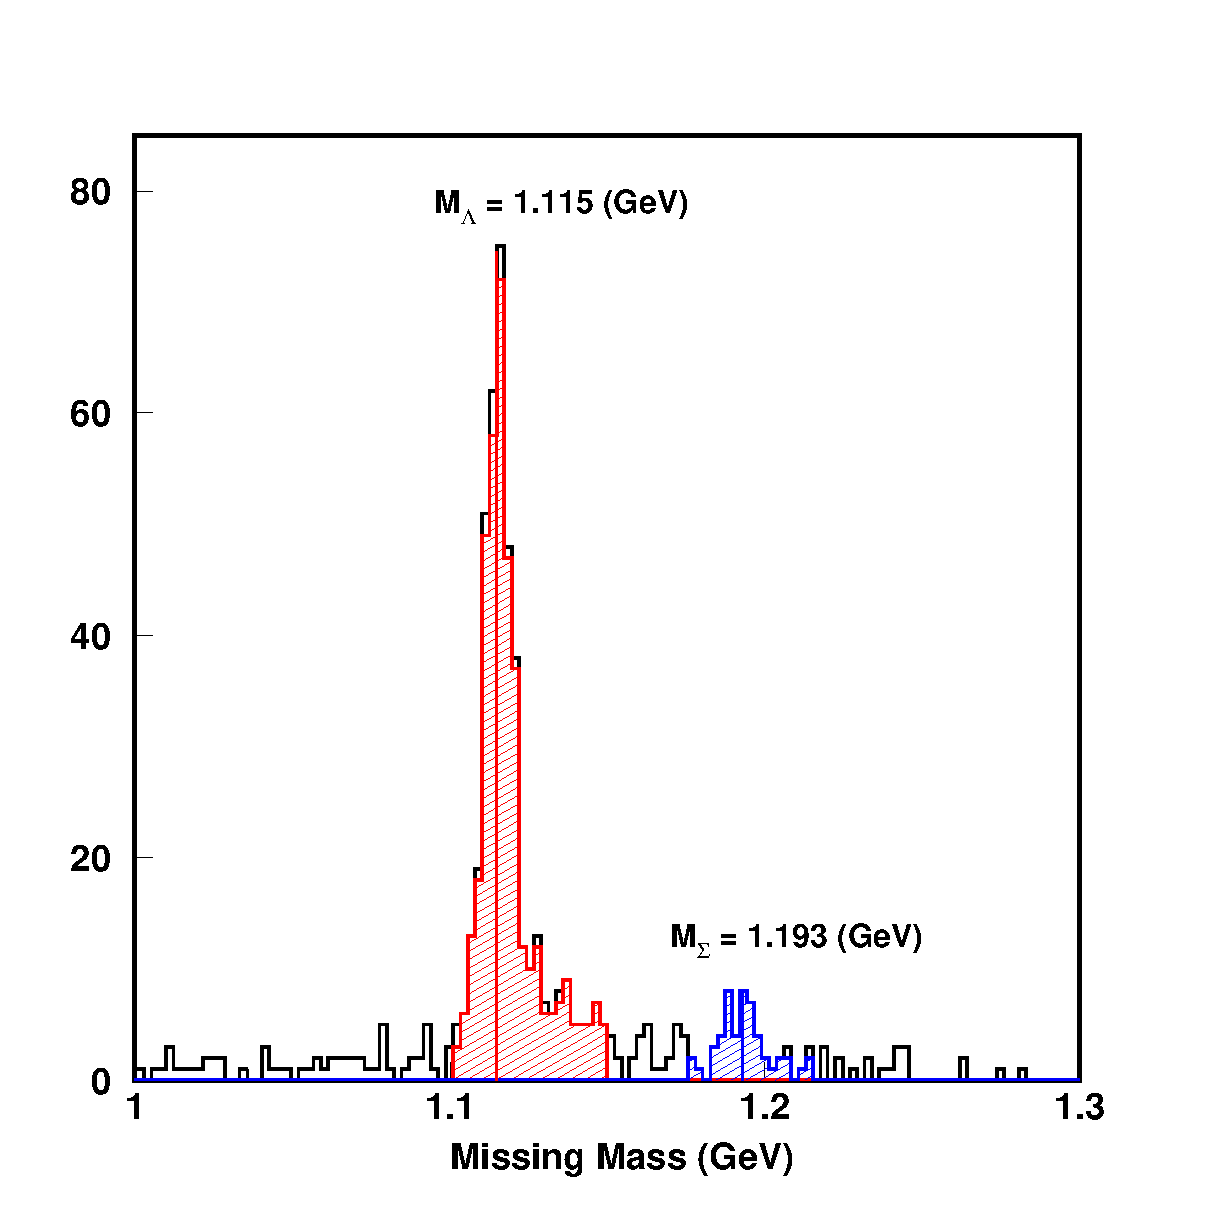
\includegraphics[width=0.8\columnwidth]{missmass1}
  \caption[One-dimensional missing mass plot.]{\label{fig:missmass1}One-dimensional missing mass plot.\\\\ First sharp peak is due to $\Lambda$ production and second small peak is due to $\Sigma$ production of kaons.}
\end{figure}
%\setlength{\figwidth}{0.8\linewidth}
%\Figure{missmass1}{\figwidth}{One-dimensional missing mass plot. First sharp peak is due to $\Lambda$ and second small peak is due to $\Sigma^0$.}

%\setlength{\figwidth}{1.0\linewidth}
%\Figure{missmass2}{\figwidth}{One dimensional plot of missing mass are shown here after applying cuts. Clockwise top left corner: $M_\Lambda^{SIMC}$, $M_\Sigma^{SIMC}$, $M_\Sigma^{data}$ and $M_\Lambda^{data}$}

\begin{figure}[!tbp]
  \centering
  \includegraphics[width=0.8\columnwidth]{com_plot_missmass_2}
  \caption[One-dimensional missing mass plot after applying cuts.]{\label{fig:com_plot_missmass_2}One-dimensional missing mass plot after applying cuts.\\\\ $M_\Lambda^{SIMC}$ and $M_\Sigma^{SIMC}$ are shown in RED and $M_\Sigma^{data}$ and $M_\Lambda^{data}$ are in BLUE.}
\end{figure}
%\setlength{\figwidth}{0.8\linewidth}
%\Figure{com_plot_missmass_2}{\figwidth}{One-dimensional plot of missing mass is shown here after applying cuts. $M_\Lambda^{SIMC}$ and $M_\Sigma^{SIMC}$ are shown in \textcolor{red}{RED} and $M_\Sigma^{data}$ and $M_\Lambda^{data}$ are in \textcolor{blue}{BLUE}.}

\begin{figure}[!tbp]
  \centering
  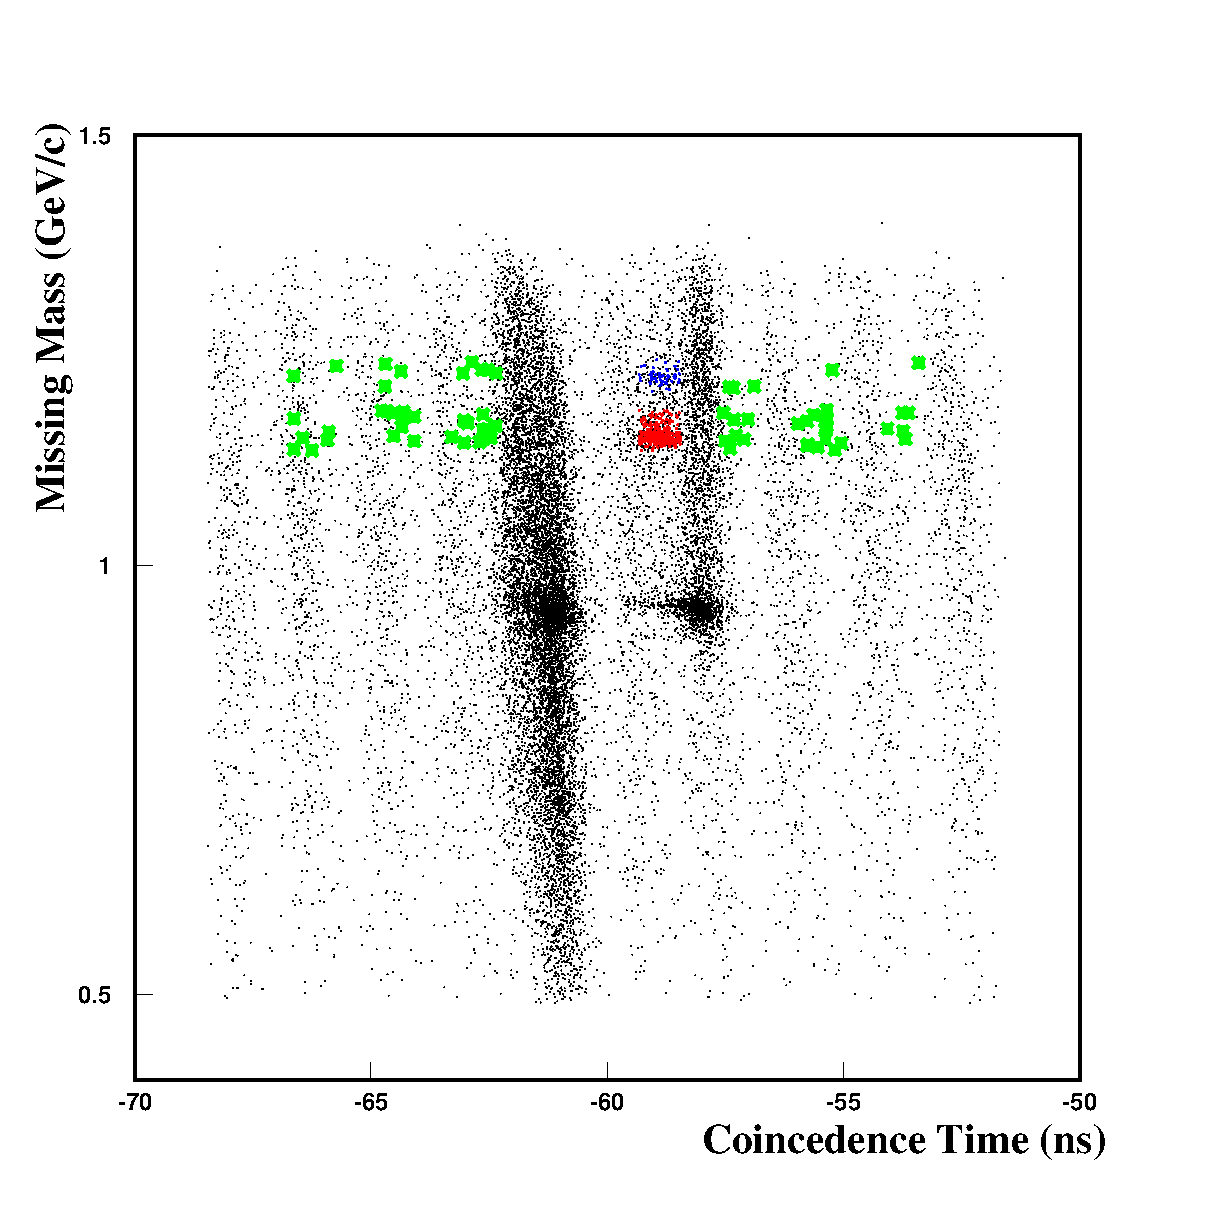
\includegraphics[trim = 3mm 3mm 3mm 3mm,clip,width=0.8\columnwidth]{misscoin}
  \caption[Two-dimensional plot of missing mass vs coincidence time.]{\label{fig:misscoin}Two-dimensional plot of missing mass vs coincidence time.\\\\ p, $K^+$ and $\pi^+$ are shown here from left to right, respectively, after applying loose cuts.}
\end{figure}
%\setlength{\figwidth}{0.8\linewidth}
%\Figure{misscoin}{\figwidth}{Two-dimensional plot of missing mass vs coincidence time. p, $K^+$ and $\pi^+$ are shown here from left to right, respectively, after applying loose cuts.}

Using the missing mass variable for hydrogen data, we have separated $K^+$ from $\Lambda$ and $\Sigma$ production. From these events, we determine a ratio of $\frac{\Lambda}{\Sigma}$.We used this same ratio in the Monte Carlo simulation. In targets heavier than hydrogen, the Fermi motion\footnote{The quantum motion of nucleons bound inside a nucleus is knwon as Fermi motion.} of the nucleons begin to broaden the $\Lambda$ and $\Sigma$ peak and are very difficult to distinguish. For all other targets due to the spreading of $\Lambda$ and $\Sigma$, we used a single cut over both $\Lambda$ and $\Sigma$ masses to separate $K^+$.

The missing mass spectrum shown in \figureref{missmass1} is from the hydrogen target for $Q^2$ = 1.1 $(\mathrm{GeV/c})^2$. In \figureref{missmass1}, the BLACK region represents events without any cut and the RED region represents the application of the cut on missing mass for $K^+$ production from $\Lambda$ and BLUE shows from the $\Sigma$ channel, whereas the RED vertical line at $M_\Lambda$ = 1.115 $(\mathrm{GeV/c})^2$ shows the mass of $\Lambda$ and BLUE vertical line at $M_\Sigma$ = 1.193 $(\mathrm{GeV/c})^2$ shows the mass of $\Sigma$ from \cite{PDG}. For $\Sigma$ mass we have taken average of the mass of $\Sigma^0$ and $\Sigma^-$ since we have two $\Sigma$ channels; given our meagre statistics, we are unable to separate $\Sigma^0$ and $\Sigma^-$ productions.

The missing mass variable is shown in \figureref{com_plot_missmass_2} after applying all the cuts where the SIMC yields are shown by RED and data by BLUE. $\Lambda$ and $\Sigma$ production have been separated by using the hydrogen data. \figureref{misscoin} shows two-dimensional plot of missing mass vs coincidence time. The $\Lambda$ events are shown in RED and $\Sigma$ in BLUE.

\begin{figure}[!tbp]
  \centering
  \includegraphics[width=0.8\columnwidth]{pid1}
  \caption[Aerogel $\breve{C}$erenkov detector.]{\label{fig:pid1}Aerogel $\breve{C}$erenkov detector.\\\\ Proton, pion and kaon thresholds for producing $\breve{C}$erenkov radiation in the aerogel $\breve{C}$erenkov detector are shown by RED, GREEN and BLUE curves respectively.}
\end{figure}
%\setlength{\figwidth}{0.8\linewidth}
%\Figure{pid1}{\figwidth}{Aerogel $\breve{C}$erenkov detector: Proton, pion and kaon thresholds for producing $\breve{C}$erenkov radiation in the aerogel $\breve{C}$erenkov detector are shown by \textcolor{red}{RED}, \textcolor{green}{GREEN} and \textcolor{blue}{BLUE} curves respectively.}

\begin{figure}[!tbp]
  \centering
  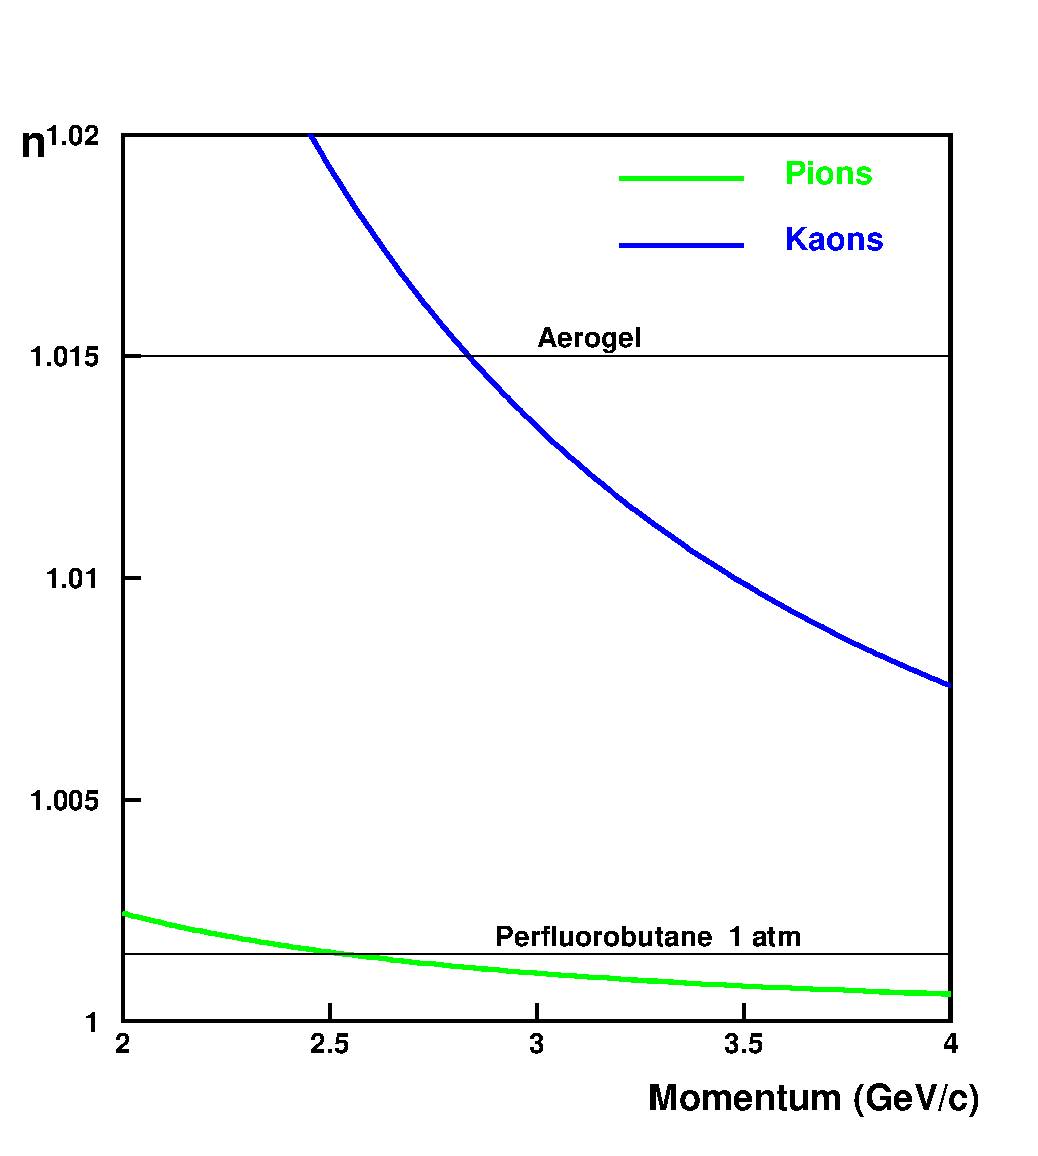
\includegraphics[width=0.8\columnwidth]{pid2}
  \caption[Gas $\breve{C}$erenkov detector.]{\label{fig:pid2}Gas $\breve{C}$erenkov detector.\\\\ Kaon and pion thresholds for producing $\breve{C}$erenkov radiation in the gas $\breve{C}$erenkov detector are shown by BLUE and GREEN curves, respectively.}
\end{figure}
%\setlength{\figwidth}{0.8\linewidth}
%\Figure{pid2}{\figwidth}{Gas $\breve{C}$erenkov detector: Kaon and pion thresholds for producing $\breve{C}$erenkov radiation in the gas $\breve{C}$erenkov detector are shown by \textcolor{blue}{BLUE} and \textcolor{green}{GREEN} curves, respectively.}

\SubSection{$\breve{C}$erenkov Radiation}%
%\label{$\breve{C}$erenkov}%
%Two type of $\breve{C}$erenkov i.e,. Aerogel and Gas $\breve{C}$erenkov have been used to identify particles in the experiment. The aerogel $\breve{C}$erenkov used in the experiment has a refractive index of n=1.015. In \figureref{pid1} the threshold for firing aerogel $\breve{C}$erenkov for proton, pion and kaon are shown in the \textcolor{red}{RED}, \textcolor{blue}{BLUE} and PURPPLE curve respectively. It is clear that protons never fire the aerogel and except for kinematics of $Q^2$ of 1.1 $GeV^2$ pion also do not fire, where as kaon always fire the aerogel. By applying a constraint over the aerogel we can seperate protons and pions from kaons. For the $Q^2$ of 1.1 $GeV^2$ kinematics, the aerogel can separete protons from pions and kaons. 
Two type of $\breve{C}$erenkov detectors, i.e, aerogel and gas $\breve{C}$erenkov, have been used to identify particles in the experiment. The aerogel $\breve{C}$erenkov detector used in the experiment has a refractive index of n = 1.015. In \figureref{pid1} we show the threshold for producing $\breve{C}$erenkov radiation by proton (RED curve), pions (GREEN curve), and kaons (BLUE curve). From this figure, we see that in our experiment the protons never produce $\breve{C}$erenkov radiation in the aerogel detector because the proton momentum in the experiment ($P_p$ = 2.7 - 3.4 $(GeV/c)$) is always above the threshold, while the kaons produce $\breve{C}$erenkov radiation for all kinematics except the $Q^2$ = 1.1 $(GeV/c)^2$ kinematics where the kaon momentum is $P_K$ = 2.7 $(GeV/c)$ which is above threshold for the aerogel. The pions are always below threshold and produce $\breve{C}$erenkov radiation for all kinematics. By applying cuts on the number of photo-electrons detected in the aerogel detector we could separate the protons from kaons and pions at all kinematics except $Q^2$ = 1.1 $(GeV/c)^2$. 

The gas $\breve{C}$erenkov detector uses perflurobutane at 1 atmosphere which has a refractive index of 1.0015. In \figureref{pid1}, the thresholds for pion and kaon are being shown by GREEN and BLUE curve, respectively. Kaons could be separated from pions by cutting on gas $\breve{C}$erenkov signal. If we apply cuts on the gas $\breve{C}$erenkov signal, then we will be able to separate kaons from pions. So, applying cuts on the two $\breve{C}$erenkov detectors we could separate kaons from pions and protons.

\Section{Cuts}
\label{Cuts}
The cuts applied on the reconstructed variables are shown in \tableref{cuts}. The cuts applied on data and the SIMC yields were the same for all cases. We have applied very tight cuts on all the variables to restrict the data to regions where the shape of that variable matches with SIMC yields.

\begin{table}
  \caption[Cuts applied on the reconstructed variables for data or SIMC.]{\label{tab:cuts}Cuts applied on the reconstructed variables for data or SIMC.}
\begin{center}
\begin{tabular}{||c|c|c||}\hline
 Variables & Left & Right \\
 & & \\\hline
Coincidence Time & -59.21 & -58.13 \\
$Missing Mass_\Lambda$ & 1.10 & 1.15 \\
$Missing Mass_\Sigma$ & 1.175 & 1.215 \\\hline
hsxptar & -0.075 & 0.075 \\
hsyptar & -0.03 & 0.03 \\
hsdelta & -10 & 5 \\
ssxptar & -0.065 & 0.065 \\
ssyptar & -0.0375 & 0.0375 \\
ssdelta & -18 & 5 \\\hline
$Q^2$ & 1.4 & 2.5 \\
W & 2.18 & 2.48 \\
t & 0.23 & 0.52 \\
$\phi_{pq}$ & 1.5 & 5 \\\hline
\end{tabular}
\end{center}
\end{table}
%\Table{cuts}{Cuts applied on the reconstructed variables for data or SIMC yields for kinematics of $Q^2$= 2.2 $(\mathrm{GeV/c})^2$.}

The cuts applied on data or SIMC yields for kinematics of $Q^2$= 2.2 $(\mathrm{GeV/c})^2$ have been shown in \tableref{cuts}. Most of the cuts applied on all the variables were quite similar for all the kinematics. We separated $\Lambda$ and $\Sigma$ production of $K^+$ for hydrogen data for all the variables. As we went to the heavier targets, the regions for $\Lambda$ and $\Sigma$ production seems to merge for almost all the variables and hence we were not able to separate them. So, the cuts applied for all other targets were similar with each other except for hydrogen.

\SubSection{Other Cuts}%
%
\label{Other Cuts}
Cuts were applied on several other reconstructed variables, such as \textit{hsxptar}, \textit{hsyptar}, \textit{ssxptar}, \textit{ssyptar}, \textit{hsdelta}, \textit{ssdelta}, etc., which define the feducial acceptance of the detector. These cuts have been applied to restrict the data to regions where they match the simulation. These cuts were discussed in the previous chapter.

%We have used several other PIDs like: hsxptar, hsyptar, ssxptar, ssyptar, hsdelta, ssdelta, hsbeta etc. Giving cuts over these PIDs we able to seperate different hadrons as well as reduce the background. As we had a very low stastictics, for thses other PIDs I applied very tight cut. The information that were avilable in the SIMC, I considered only that region. Means giving a very tight cut cosidered the common region for data and SIMC.

\Section{Comparison of Data with SIMC Yields}%
%
\label{Comparison of Data with SIMC Yields}
The cross section depends upon four variables; they are $Q^2$, $W$, $t$, $\phi_{pq}$, where $Q^2$ is four- momentum transferred square, $W$ is the C.M. energy, $t$ is momentum transfer, and $\phi_{pq}$ is  the angle between the scattering and reaction planes. So before calculating transparency, we compare the data with SIMC yields for these variables. If the simulated shape of these variables agree with the data, we can claim that the model used in the SIMC simulation is valid. After adding $\Lambda$ and $\Sigma$ production for $K^+$ with proper ratio obtained using hydrogen data, the yields are shown in \figureref{com_plot_2_Q2_2} for variable $Q^2$. The same procedure was applied to other variables as well. Comparison of data yields and SIMC yields for the variables $W$, $t$ and $\phi_{pq}$ after adding $\Lambda$ and $\Sigma$ production for $K^+$ are shown in \figureref{com_plot_2_w_2}, \figureref{com_plot_2_t_2} and  \figureref{com_plot_2_phi_2}, respectively.

\begin{figure}[!tbp]
  \centering
  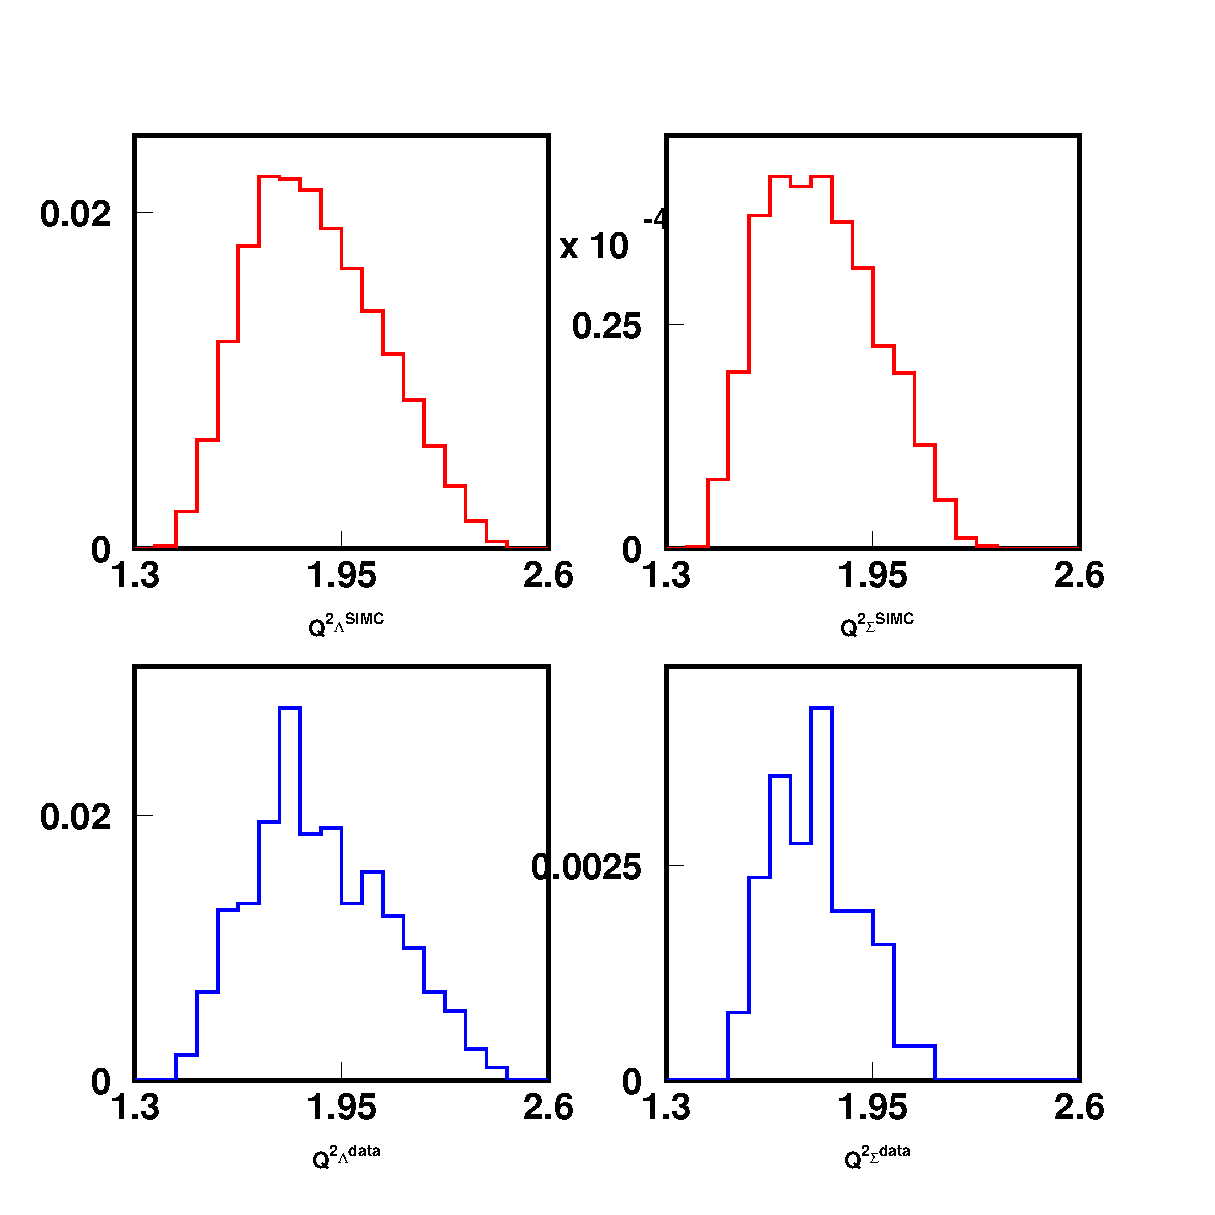
\includegraphics[width=0.8\columnwidth]{Q2_1}
  \caption[Comparison of $Q^2$ from data and SIMC.]{\label{fig:Q2_1}Comparison of $Q^2$ from data and SIMC.\\\\ Clockwise from top left corner: $Q^2_\Lambda$ SIMC, $Q^2_\Sigma$ SIMC, $Q^2_\Sigma$ data, $Q^2_\Lambda$ data for $Q^2$=2.2 $(\mathrm{GeV/c})^2$, where SIMC and data are shown in RED and BLUE, respectively.}
\end{figure}
%\setlength{\figwidth}{0.8\linewidth}
%\Figure{Q2_1}{\figwidth}{$Q^2$. Clockwise from top left corner: $Q^2_\Lambda$ SIMC, $Q^2_\Sigma$ SIMC, $Q^2_\Sigma$ data, $Q^2_\Lambda$ data for $Q^2$=2.2 $(\mathrm{GeV/c})^2$, where SIMC and data are shown in \textcolor{red}{RED} and \textcolor{blue}{BLUE}, respectively.}

%\setlength{\figwidth}{0.8\linewidth}
%\Figure{Q2_2}{\figwidth}{$Q^2$ combined $\Lambda$ and $\Sigma$ for both SIMC and data in \textcolor{red}{RED} and \textcolor{blue}{BLUE} respectively for $Q^2$=2.2 $GeV^2$}
\begin{figure}[!tbp]
  \centering
  \includegraphics[width=0.8\columnwidth]{com_plot_2_Q2_2}
  \caption[Comparison of $Q^2$ from data and SIMC.]{\label{fig:com_plot_2_Q2_2}Comparison of $Q^2$ from data and SIMC.\\\\ $Q^2$ combined $\Lambda$ and $\Sigma$ for both SIMC and data yields in RED and BLUE respectively for $(\mathrm{GeV/c})^2$.}
\end{figure}
%\setlength{\figwidth}{0.8\linewidth}
%\Figure{com_plot_2_Q2_2}{\figwidth}{$Q^2$ combined $\Lambda$ and $\Sigma$ for both SIMC and data yields in \textcolor{red}{RED} and \textcolor{blue}{BLUE} respectively for $(\mathrm{GeV/c})^2$.}

%\setlength{\figwidth}{0.8\linewidth}
%\Figure{w_1}{\figwidth}{W. Clockwise from top left corener: $W_\Lambda$ SIMC, $W_\Sigma$ SIMC, $W_\Sigma$ data, $W_\Lambda$ data for $Q^2$=2.2 $GeV^2$}
\begin{figure}[!tbp]
  \centering
  \includegraphics[width=0.8\columnwidth]{com_plot_2_w_2}
  \caption[Comparison of $W$ from data and SIMC.]{\label{fig:com_plot_2_w_2}Comparison of $W$ from data and SIMC.\\\\ $W$ combined $\Lambda$ and $\Sigma$ for both SIMC and data yields in RED and BLUE, respectively, for $Q^2$=2.2 $(\mathrm{GeV/c})^2$.}
\end{figure}
%\setlength{\figwidth}{0.8\linewidth}
%\Figure{com_plot_2_w_2}{\figwidth}{$W$ combined $\Lambda$ and $\Sigma$ for both SIMC and data yields in \textcolor{red}{RED} and \textcolor{blue}{BLUE}, respectively, for $Q^2$=2.2 $(\mathrm{GeV/c})^2$.}

%\setlength{\figwidth}{0.8\linewidth}
%\Figure{t_1}{\figwidth}{t. Clockwise from top left corener: $t_\Lambda$ SIMC, $t_\Sigma$ SIMC, $t_\Sigma$ data, $t_\Lambda$ data for $Q^2$=2.2 $GeV^2$}
\begin{figure}[!tbp]
  \centering
  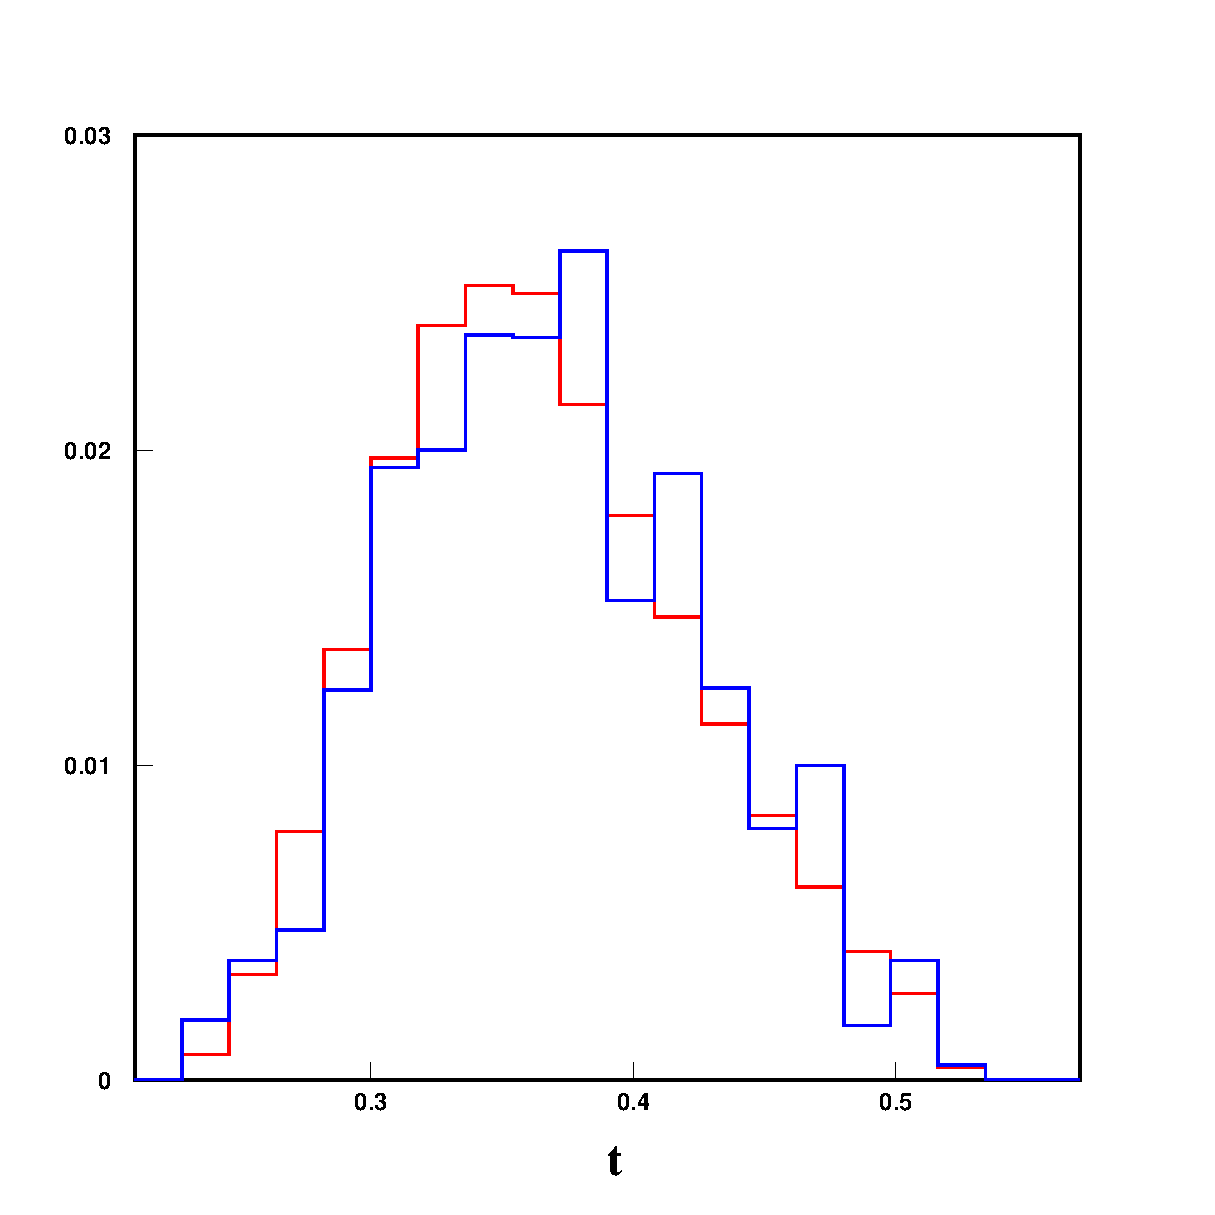
\includegraphics[width=0.8\columnwidth]{com_plot_2_t_2}
  \caption[Comparison of $t$ from data and SIMC.]{\label{fig:com_plot_2_t_2}Comparison of $t$ from data and SIMC.\\\\ $t$ combined $\Lambda$ and $\Sigma$ for both SIMC and data yields in RED and BLUE, respectively, for $Q^2$=2.2 $(\mathrm{GeV/c})^2$.}
\end{figure}
%\setlength{\figwidth}{0.8\linewidth}
%\Figure{com_plot_2_t_2}{\figwidth}{$t$ combined $\Lambda$ and $\Sigma$ for both SIMC and data yields in \textcolor{red}{RED} and \textcolor{blue}{BLUE}, respectively, for $Q^2$=2.2 $(\mathrm{GeV/c})^2$.}

%\setlength{\figwidth}{0.8\linewidth}
%\Figure{phipq_1}{\figwidth}{$\phi^{pq}$. Clockwise from top left corener: $\phi^{pq}_\Lambda$ SIMC, $\phi^{pq}_\Sigma$ SIMC, $\phi^{pq}_\Sigma$ data, $\phi^{pq}_\Lambda$ data for $Q^2$=2.2 $GeV^2$}
\begin{figure}[!tbp]
  \centering
  \includegraphics[width=0.8\columnwidth]{com_plot_2_phi_2}
  \caption[Comparison of $\phi_{pq}$ from data and SIMC.]{\label{fig:com_plot_2_phi_2}Comparison of $\phi_{pq}$ from data and SIMC.\\\\ $\phi_{pq}$ combined $\Lambda$ and $\Sigma$ for both SIMC and data yields in RED and BLUE, respectively, for $Q^2$=2.2 $(\mathrm{GeV/c})^2$.}
\end{figure}
%\setlength{\figwidth}{0.8\linewidth}
%\Figure{com_plot_2_phi_2}{\figwidth}{$\phi_{pq}$ combined $\Lambda$ and $\Sigma$ for both SIMC and data yields in \textcolor{red}{RED} and \textcolor{blue}{BLUE}, respectively, for $Q^2$=2.2 $(\mathrm{GeV/c})^2$.}